\documentclass[10pt,journal,compsoc]{IEEEtran}

\usepackage{amsmath,amssymb,amsfonts}
\usepackage{algorithmic}
\usepackage{graphicx}
\usepackage{textcomp}
\usepackage{xcolor}
\usepackage{booktabs}
\usepackage{multirow}
\usepackage{tabularx}
\usepackage{hyperref}
\usepackage{url}
\usepackage{cite}
\usepackage{balance}
\usepackage{pifont}
\usepackage{enumitem}

\hypersetup{
    colorlinks=true,
    linkcolor=blue!70!black,
    citecolor=blue!70!black,
    urlcolor=blue!70!black
}

\newcommand{\cmark}{\ding{51}}
\newcommand{\xmark}{\ding{55}}

\begin{document}

\title{Large Language Models and Foundation Models for Time Series: A Survey and Outlook}

\author{Huirui~Li
\IEEEcompsocitemizethanks{
\IEEEcompsocthanksitem H. Li is the sole author and maintainer of this living survey repository. Contact: 58367737+lihuirui@users.noreply.github.com. Project repository: \url{https://github.com/lihuirui/awesome-llm-time-series-foundation-models-survey}.
}
}

\IEEEtitleabstractindextext{
\begin{abstract}
Time series analysis underpins mission-critical decision systems across modern society, including industrial Internet of Things (IoT), computational finance, energy grid stabilization, meteorological forecasting, and clinical healthcare. Over the past five years, the field has undergone a profound paradigm shift from narrow, task-specific deep neural networks (such as specialized LSTMs and convolutional architectures) toward scalable foundation models. This evolution is bifurcated into two dominant architectural philosophies: (1) \emph{Native Time Series Foundation Models (TSFMs)}, which are trained ab initio on massive cross-domain time-series corpora comprising tens to hundreds of billions of observations (e.g., Chronos, TimesFM, MOIRAI, MOMENT, Lag-Llama, TTM, Timer, Sundial, Time-MoE, and Toto); and (2) \emph{Repurposed Large Language Models (LLM4TS)}, which repurpose frozen or parameter-efficiently adapted language transformers to temporal sequences through cross-modal token reprogramming, decimal prompting, or multimodal instruction tuning (e.g., Time-LLM, GPT4TS/OFA, LLMTime, TEMPO, and S2IP-LLM). In this survey, conducted strictly under the PRISMA 2020 systematic review protocol, we provide the first unified, comprehensive taxonomy and comparative synthesis spanning 2021 through 2026. We formalize the mathematical preliminaries of temporal representation, deconstruct core tokenization mechanics (patching vs. scalar quantization vs. lag vectors), analyze probabilistic formulation heads, examine empirical scaling behaviors and zero-shot transfer capabilities, and critically evaluate the central debate: \emph{Are billion-parameter language backbones truly necessary, or do compact specialized foundation models provide superior accuracy and operational efficiency?} Finally, we conduct an audit of standardized benchmarks (e.g., GIFT-Eval), uncover evaluation pitfalls such as benchmark contamination and temporal leakage, and delineate open research directions toward multi-modal temporal intelligence.
\end{abstract}

\begin{IEEEkeywords}
Time series analysis, foundation models, large language models, deep learning, zero-shot forecasting, tokenization, scaling laws, PRISMA systematic review.
\end{IEEEkeywords}}

\maketitle
\IEEEdisplaynontitleabstractindextext
\IEEEpeerreviewmaketitle

\section{Introduction}
\label{sec:intro}

\IEEEPARstart{T}{emporal} data, systematically recorded as univariate or multivariate time series, serves as the fundamental perceptual substrate for understanding dynamic physical, economic, and biological systems. Across modern industries, time series forecasting, anomaly detection, imputation, and classification drive mission-critical workflows: stabilizing renewable energy power grids, optimizing multi-echelon retail supply chains, executing high-frequency financial risk arbitrage, predicting clinical sepsis in intensive care units, and monitoring aerospace telemetry~\cite{jin2023largemodels}.

Historically, time series modeling evolved through three distinct algorithmic epochs:
\begin{enumerate}[leftmargin=*]
    \item \emph{Statistical and Econometric Formulation (1970s--2010s)}: Dominated by classical stochastic processes, such as Auto-Regressive Integrated Moving Average (ARIMA), Exponential Smoothing (ETS), Vector Autoregression (VAR), and Gaussian Processes. While mathematically rigorous and interpretable, these methods rely on linear assumptions and fail to capture complex nonlinear dependencies across cross-domain series.
    \item \emph{Task-Specific Deep Neural Networks (2015--2022)}: Catalyzed by recurrent architectures (LSTMs, GRUs), temporal convolutional networks (TCNs), and specialized Transformer variants (Informer, Autoformer, FEDformer, and PatchTST~\cite{nie2023patchtst}). Although these architectures captured long-range nonlinear temporal correlations, each model was trained in isolation on a single, isolated dataset (e.g., ETT, Weather, Electricity), exhibiting virtually zero out-of-distribution generalization.
    \item \emph{The Foundation Model Epoch (2022--Present)}: Propelled by the extraordinary success of pre-trained foundation models in Natural Language Processing (e.g., GPT-4, Llama) and Computer Vision, the temporal machine learning community has initiated a paradigm shift toward universal, cross-domain foundation models~\cite{ansari2024chronos,das2024timesfm,woo2024moirai}. Rather than training narrow models from scratch for every new dataset, practitioners now seek models capable of strong zero-shot and few-shot transfer across unseen domains, frequencies, and channels.
\end{enumerate}

\subsection{Unique Challenges of Temporal Signals}
Transferring the foundation model paradigm to time series is non-trivial due to stark physical and mathematical differences between temporal signals and natural language:
\begin{itemize}[leftmargin=*]
    \item \emph{Absence of a Discrete Natural Vocabulary}: Unlike natural text, which is composed of finite, discrete lexical tokens with stable semantic meanings, continuous time series $\mathbf{x} \in \mathbb{R}^T$ consist of real-valued scalar measurements bounded only by sensor physics.
    \item \emph{Extreme Heterogeneity in Sampling Rates and Dynamics}: Real-world time series exhibit widely divergent temporal scales—ranging from milliseconds in financial order books, to hourly power consumption, to daily retail demand, to quarterly economic indicators. A model must reconcile varying seasonalities without destructive aliasing.
    \item \emph{Variable Dimensionality and Missing Values}: Time series data dynamically switch between univariate streams and arbitrary multivariate configurations ($C \ge 1$), frequently accompanied by irregular observation intervals, sensor failure dropouts, and structural trend shifts.
\end{itemize}

\begin{table*}[t]
\caption{Comparison of This Survey with Related Surveys on Large Temporal Models.}
\label{tab:survey_comparison}
\centering
\small
\begin{tabularx}{\textwidth}{lcccccX}
\toprule
\textbf{Survey Reference} & \textbf{Year} & \textbf{PRISMA} & \textbf{Native TSFMs} & \textbf{Repurposed LLMs} & \textbf{Critiques \& Audits} & \textbf{Primary Focus \& Distinguishing Scope} \\
\midrule
Wen et al.~\cite{jin2023largemodels} & 2023 & \xmark & \xmark & \xmark & \xmark & Survey of specialized Transformer architectures on single datasets. \\
Jin et al.~\cite{jin2023largemodels} & 2024 & \xmark & Partial & \cmark & Partial & Broad survey covering both general time series and spatio-temporal graphs. \\
Gruver et al.~\cite{gruver2023llmtime} & 2023 & \xmark & \xmark & \cmark & \xmark & Empirical investigation of prompting LLMs as zero-shot forecasters. \\
Fons et al.~\cite{fons2024arellmsuseful} & 2024 & \xmark & \xmark & \cmark & \cmark & Empirical critique testing whether language backbones add genuine inductive value. \\
\textbf{This Survey} & \textbf{2026} & \cmark & \cmark & \cmark & \cmark & \textbf{Comprehensive PRISMA systematic review (2021--2026); unifying Native TSFMs, Repurposed LLMs, tokenization trade-offs, scaling laws, and leakage audits.} \\
\bottomrule
\end{tabularx}
\end{table*}

\subsection{The Bifurcated Landscape: Native TSFMs vs. LLM4TS}
To address these challenges, the research community has split into two competing architectural paradigms:
\begin{enumerate}[leftmargin=*]
    \item \emph{Native Time Series Foundation Models (TSFMs)}: Architectures designed and trained from scratch on massive multi-domain temporal corpora comprising tens to hundreds of billions of observations. Prominent exemplars include Amazon Chronos~\cite{ansari2024chronos,ansari2025chronos2}, Google TimesFM~\cite{das2024timesfm,das2024incontext}, Salesforce MOIRAI~\cite{woo2024moirai,woo2024moiraimoe,woo2025moirai2}, CMU MOMENT~\cite{goswami2024moment}, IBM TTM~\cite{ekambaram2024ttm}, Morgan Stanley/Mila Lag-Llama~\cite{rasul2023lagllama}, and the THUML Timer family~\cite{liu2024timer,liu2024timerxl,thuml2025sundial,thuml2026timers1}.
    \item \emph{Repurposed Large Language Models (LLM4TS)}: Approaches that leverage the pre-trained weights, attention layers, and sequence modeling capabilities of multi-billion parameter language models (such as Llama, GPT-2, or GPT-4). Techniques include cross-modal token reprogramming (e.g., Time-LLM~\cite{jin2023timellm}, GPT4TS/OFA~\cite{zhou2023onefitsall}, TEMPO~\cite{cao2023tempo}), direct numeric prompting with ASCII decimal strings (e.g., LLMTime~\cite{gruver2023llmtime}), and multimodal question-answering agents (e.g., Time-MQA~\cite{jin2025timemqa}, TimeOmni-1~\cite{jin2025timeomni}).
\end{enumerate}

\subsection{Key Contributions of This Survey}
While several initial surveys have examined aspects of deep learning for time series, the rapid surge of foundation models from 2024 to 2026 demands a rigorous, systematic, and up-to-date synthesis. As highlighted in Table~\ref{tab:survey_comparison}, this work delivers the following contributions:
\begin{enumerate}[leftmargin=*]
    \item \emph{PRISMA 2020 Systematic Review Protocol}: We execute a strictly reproducible review protocol across scholarly APIs, logging 83 initial records, screening against standardized criteria, and synthesizing 41 core benchmark and foundation models.
    \item \emph{Rigorous Unified Taxonomy}: We establish an orthogonal five-dimensional taxonomy deconstructing models along: (i) architectural backbone, (ii) temporal tokenization, (iii) prediction head and uncertainty formulation, (iv) adaptation mechanics, and (v) operational task scope.
    \item \emph{Deep Comparative Synthesis of Native TSFMs vs. LLM4TS}: We analyze the theoretical and empirical tensions between compact native models ($1\text{M}$--$700\text{M}$ parameters) and multi-billion parameter language adaptations ($7\text{B}$--$70\text{B}$ parameters), examining computational efficiency, inference latency, and inductive bias alignment.
    \item \emph{Benchmark Audit, Data Contamination, and Scaling Laws}: We survey modern evaluation suites (e.g., GIFT-Eval~\cite{salesforce2024gifteval}), expose systemic data leakage risks~\cite{gong2025rethinkingeval}, analyze empirical power-law scaling in temporal models, and assess probabilistic calibration reliability~\cite{li2026evaluatingreliability}.
    \item \emph{Open Research Agenda}: We articulate key open challenges, including irregular sampling equivariance, continuous flow matching, multimodal sensor fusion, and edge deployment.
\end{enumerate}

\subsection{Structure of the Survey}
The remainder of this survey is organized as follows: Section~\ref{sec:prelim} formalizes mathematical preliminaries and foundational objectives. Section~\ref{sec:taxonomy} presents our comprehensive taxonomy and comparative design table. Section~\ref{sec:native} deconstructs Native TSFMs. Section~\ref{sec:llm4ts} investigates Repurposed LLM methods. Section~\ref{sec:eval} evaluates benchmark suites, scaling laws, and critical debates. Section~\ref{sec:outlook} delineates open challenges, and Section~\ref{sec:conclusion} concludes the paper.

\section{Background and Preliminaries}
\label{sec:prelim}

In this section, we establish the formal mathematical definitions, notation, and objective functions that govern modern temporal foundation models and large language model adaptations.

\subsection{Formal Problem Definitions}

\subsubsection{Temporal Sequences}
A univariate time series of length $T$ is defined as an ordered sequence of real-valued scalar observations:
\begin{equation}
    \mathbf{x} = [x_1, x_2, \dots, x_T]^\top \in \mathbb{R}^T,
\end{equation}
where $x_t \in \mathbb{R}$ represents the measurement recorded at discrete timestamp $t \in \{1, \dots, T\}$.

A multivariate time series comprises $C$ co-evolving channels or variates observed synchronously across $T$ timestamps:
\begin{equation}
    \mathbf{X} = [\mathbf{x}^{(1)}, \mathbf{x}^{(2)}, \dots, \mathbf{x}^{(C)}]^\top \in \mathbb{R}^{C \times T},
\end{equation}
where $\mathbf{X}_{:, t} \in \mathbb{R}^C$ is the vector of all variate measurements at timestamp $t$.

\subsubsection{Channel Modeling Paradigms}
When processing multivariate series $\mathbf{X}$, architectures adopt one of two primary structural paradigms:
\begin{itemize}[leftmargin=*]
    \item \emph{Channel-Independence (CI)}: Introduced prominently in PatchTST~\cite{nie2023patchtst} and Timer~\cite{liu2024timer}, CI decomposes the multivariate series into $C$ distinct univariate sequences:
    \begin{equation}
        \mathbf{X} \mapsto \{\mathbf{x}^{(1)}, \mathbf{x}^{(2)}, \dots, \mathbf{x}^{(C)}\},
    \end{equation}
    which are fed into the shared model backbone independently with tied parameters. CI eliminates the risk of overfitting spurious cross-channel correlations and natively handles variable channel counts $C$ at inference.
    \item \emph{Channel-Mixing (CM)}: Models such as MOIRAI~\cite{woo2024moirai} and TTM~\cite{ekambaram2024ttm} employ full cross-variate attention or specialized channel-mixing MLPs:
    \begin{equation}
        \mathbf{H} = \text{Attn}_{\text{channel}}(\mathbf{X}) \in \mathbb{R}^{C \times T \times D},
    \end{equation}
    explicitly capturing physical inter-sensor dependencies at the cost of higher computational complexity.
\end{itemize}

\subsection{Tokenization and Input Representation}

Because continuous temporal values lack an inherent lexicon, models deploy specialized mapping operators $\mathcal{T}: \mathbb{R}^* \to \mathbb{R}^D$ to construct transformer-compatible token embeddings.

\subsubsection{Subseries Patching}
Rather than embedding individual scalar time-steps (which leads to quadratic attention overhead $\mathcal{O}(T^2)$ and severe information sparsity), the majority of modern TSFMs (e.g., TimesFM~\cite{das2024timesfm}, Timer~\cite{liu2024timer}, MOMENT~\cite{goswami2024moment}) partition a sequence $\mathbf{x}$ into $N$ contiguous subseries patches of length $P$ with stride $S$:
\begin{equation}
    N = \left\lfloor \frac{T - P}{S} \right\rfloor + 1.
\end{equation}
The $i$-th patch $\mathbf{p}_i = [x_{(i-1)S + 1}, \dots, x_{(i-1)S + P}]^\top \in \mathbb{R}^P$ is mapped to a $D$-dimensional latent vector $\mathbf{e}_i \in \mathbb{R}^D$ via an affine projection:
\begin{equation}
    \mathbf{e}_i = \mathbf{p}_i \mathbf{W}_p + \mathbf{b}_p + \mathbf{e}_{\text{pos}, i},
\end{equation}
where $\mathbf{W}_p \in \mathbb{R}^{P \times D}$, $\mathbf{b}_p \in \mathbb{R}^D$, and $\mathbf{e}_{\text{pos}, i} \in \mathbb{R}^D$ denotes a learnable or sinusoidal positional encoding. Patching preserves local temporal shape dynamics and compresses sequence length from $T$ to $N \ll T$.

\subsubsection{Scalar Quantization and Categorical Binning}
In contrast to continuous linear patching, Amazon Chronos~\cite{ansari2024chronos} introduces a pure language-analog tokenization. Given an input sequence $\mathbf{x}$, it computes instance-level scale statistics $(\mu, \sigma)$ via mean scaling:
\begin{equation}
    \widetilde{x}_t = \frac{x_t - \mu}{\sigma + \epsilon}, \quad \mu = \frac{1}{T}\sum_{t=1}^T x_t, \quad \sigma = \frac{1}{T}\sum_{t=1}^T |x_t - \mu|.
\end{equation}
The normalized scalars $\widetilde{x}_t$ are discretized into $K$ uniform bins over $[-B, B]$:
\begin{equation}
    q_t = \text{clip}\left(\left\lfloor \frac{\widetilde{x}_t - (-B)}{2B / K} \right\rfloor, 0, K - 1\right),
\end{equation}
where $q_t \in \{0, 1, \dots, K-1\}$ acts as a discrete categorical token id, enabling standard cross-entropy language modeling.

\subsection{Downstream Task Formulations}

\subsubsection{Zero-Shot and Supervised Forecasting}
Given an historical context window $\mathbf{X}_{1:T} \in \mathbb{R}^{C \times T}$, the forecasting objective is to predict the future sequence of length $H$:
\begin{equation}
    \widehat{\mathbf{Y}} = \widehat{\mathbf{X}}_{T+1:T+H} \in \mathbb{R}^{C \times H}.
\end{equation}
In \emph{probabilistic forecasting}, the model estimates the conditional predictive distribution:
\begin{equation}
    p(\mathbf{Y} \mid \mathbf{X}_{1:T}) = \prod_{h=1}^H p(y_{T+h} \mid \mathbf{X}_{1:T}, y_{T+1:T+h-1}).
\end{equation}
This distribution is parameterized either parametrically (e.g., Student's $t$ parameters in Lag-Llama~\cite{rasul2023lagllama} or Gaussian mixtures in MOIRAI~\cite{woo2024moirai}) or non-parametrically through categorical bin logits (Chronos~\cite{ansari2024chronos}).

\subsection{Pre-training Objectives}

\subsubsection{Autoregressive Generation (Next-Patch / Next-Token)}
Decoder-only foundation models (TimesFM~\cite{das2024timesfm}, Timer~\cite{liu2024timer}, Chronos~\cite{ansari2024chronos}) optimize an autoregressive likelihood:
\begin{equation}
    \mathcal{L}_{\text{AR}}(\Theta) = -\sum_{i=1}^N \log p_\Theta(\mathbf{p}_{i+1} \mid \mathbf{p}_1, \dots, \mathbf{p}_i).
\end{equation}
For continuous regression heads (Timer, TimesFM), this is computed using Mean Squared Error (MSE) or Mean Absolute Error (MAE):
\begin{equation}
    \mathcal{L}_{\text{reg}}(\Theta) = \frac{1}{N} \sum_{i=1}^N \|\mathbf{p}_{i+1} - \widehat{\mathbf{p}}_{i+1}\|_2^2.
\end{equation}

\subsubsection{Masked Autoencoding (MAE)}
Encoder-based foundation models (MOMENT~\cite{goswami2024moment}, PatchTST~\cite{nie2023patchtst}) apply a binary masking vector $\mathbf{m} \in \{0, 1\}^N$ over patches, optimizing patch reconstruction over the masked set $\mathcal{M} = \{i \mid m_i = 1\}$:
\begin{equation}
    \mathcal{L}_{\text{Mask}}(\Theta) = \frac{1}{|\mathcal{M}|} \sum_{i \in \mathcal{M}} \|\mathbf{p}_i - f_\Theta(\mathbf{X}_{\backslash \mathcal{M}})\|_2^2.
\end{equation}
Masked autoencoding yields bidirectional temporal representations particularly suited for downstream classification, anomaly detection, and imputation.

\section{Taxonomy and Landscape Overview}
\label{sec:taxonomy}

To organize the rapid proliferation of temporal foundation models and large language model adaptations, we present an orthogonal multi-dimensional taxonomy. As illustrated in Figure~\ref{fig:taxonomy_overview}, the landscape is structured along five fundamental axes: (1) Core Paradigm, (2) Architectural Backbone, (3) Temporal Tokenization, (4) Prediction Head \& Uncertainty, and (5) Operational Scope \& Tasks.

\begin{figure*}[t]
\centering
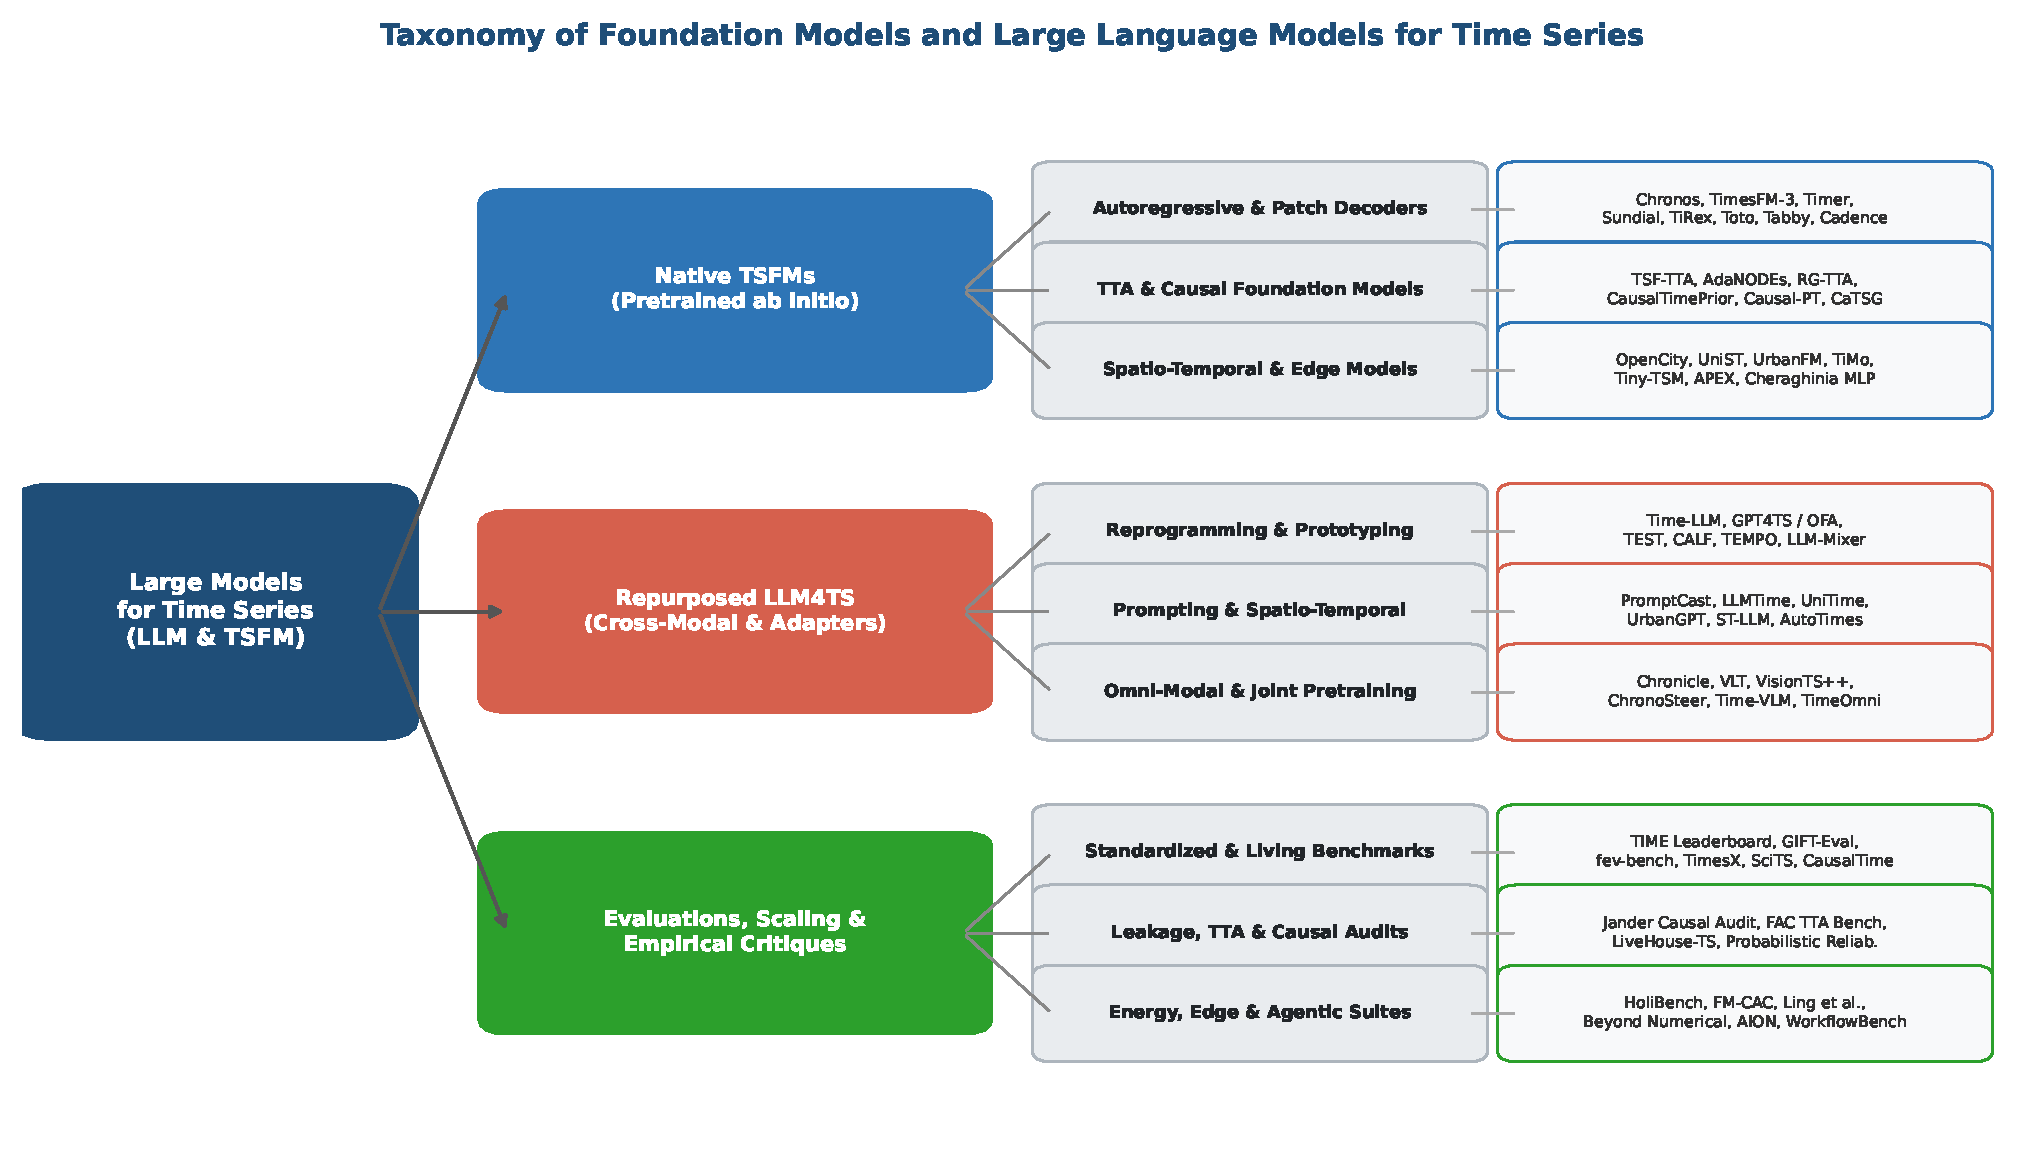
\includegraphics[width=0.98\textwidth]{figures/fig_taxonomy.pdf}
\caption{Comprehensive taxonomy of foundation models and large language models for time series, illustrating core paradigms, architectural backbones, tokenization mechanics, and representative models.}
\label{fig:taxonomy_overview}
\end{figure*}

\subsection{Taxonomy Dimensions}

\subsubsection{Dimension 1: Core Paradigm}
\begin{itemize}[leftmargin=*]
    \item \emph{Native Time Series Foundation Models (Native TSFMs)}: Models built from scratch and trained directly on large-scale collections of empirical or synthetic time-series data. Weights and latent dimensions are optimized specifically for temporal signals without textual preconceptions (e.g., Chronos~\cite{ansari2024chronos}, TimesFM~\cite{das2024timesfm}, MOIRAI~\cite{woo2024moirai}, ForecastPFN~\cite{dooley2023forecastpfn}, TiRex~\cite{auer2025tirex}, FLAME~\cite{wu2025flame}, $t_0$~\cite{meyer2026t0}).
    \item \emph{Repurposed Large Language Models (LLM4TS)}: Models that adopt pre-existing weights from language or vision transformers (e.g., Llama-2/3, GPT-2, CLIP), bridging continuous temporal modalities into text or visual embedding space via reprogramming layers, prompt prefixes, or cross-attention adapters (e.g., Time-LLM~\cite{jin2023timellm}, GPT4TS~\cite{zhou2023onefitsall}, TEST~\cite{sun2023test}, CALF~\cite{liu2024calf}, UniTime~\cite{liu2024unitime}, VisionTS~\cite{chen2024visionts}, Time-VLM~\cite{zhong2025timevlm}).
    \item \emph{Evaluation Frameworks and Benchmark Audits}: Standardized benchmarking suites and diagnostic harnesses that audit generalization, cross-domain transfer, and benchmark contamination (e.g., GIFT-Eval~\cite{salesforce2024gifteval}, SciTS~\cite{wu2025scits}, Insight Miner~\cite{zhang2025insightminer}, Time-MMD~\cite{yue2024timemmd}).
\end{itemize}

\subsubsection{Dimension 2: Architectural Backbone}
\begin{itemize}[leftmargin=*]
    \item \emph{Decoder-Only Autoregressive Transformers}: Optimized for sequential next-token or next-patch generation (e.g., TimesFM~\cite{das2024timesfm}, Timer~\cite{liu2024timer}, Chronos~\cite{ansari2024chronos}, Sundial~\cite{thuml2025sundial}, $t_0$~\cite{meyer2026t0}).
    \item \emph{Masked Encoder Transformers}: Optimized for bidirectional temporal representations via masked autoencoding (e.g., MOMENT~\cite{goswami2024moment}, PatchTST~\cite{nie2023patchtst}, VisionTS~\cite{chen2024visionts}).
    \item \emph{Encoder-Decoder Transformers}: Decoupling context representation from horizon generation (e.g., MOIRAI~\cite{woo2024moirai}, TTM~\cite{ekambaram2024ttm}, UniTS~\cite{zhou2024units}).
    \item \emph{Sparse Mixture-of-Experts (MoE)}: Dynamically routing tokens to specialized feed-forward experts to scale model capacity while maintaining constant inference FLOPs (e.g., Time-MoE~\cite{shi2024timemoe}, Moirai-MoE~\cite{woo2024moiraimoe}, Timer-S1~\cite{thuml2026timers1}).
    \item \emph{Continuous Flow and Legendre Memory Networks}: Employing continuous neural ODEs or orthogonal polynomial bases to preserve multi-scale memory (e.g., FLAME~\cite{wu2025flame}, FlowState~\cite{king2025flowstate}).
\end{itemize}

\subsubsection{Dimension 3: Temporal Tokenization}
\begin{itemize}[leftmargin=*]
    \item \emph{Uniform Subseries Patching}: Continuous linear projection of non-overlapping or strided time-step windows into dense embedding space (e.g., PatchTST~\cite{nie2023patchtst}, Timer~\cite{liu2024timer}).
    \item \emph{Scalar Discretization / Binning}: Quantizing scaled continuous observations into finite categorical tokens, allowing standard NLP cross-entropy training (Chronos~\cite{ansari2024chronos}).
    \item \emph{Decimal String Tokenization}: Casting continuous numbers into ASCII strings (e.g., ``12.4''), processed directly by off-the-shelf text tokenizers (PromptCast~\cite{xue2022promptcast}, LLMTime~\cite{gruver2023llmtime}).
    \item \emph{Multi-Resolution and Multiscale Mixing}: Dynamically decomposing and mixing patches across frequencies to resolve multi-scale seasonalities (TimeMixer~\cite{wang2024timemixer}, TimeMixer++~\cite{wang2024timemixerplus}, TTM~\cite{ekambaram2024ttm}).
    \item \emph{Visual Rendering Tokenization}: Rendering 1D numerical trajectories into 2D pixel line plots for visual encoders (VisionTS~\cite{chen2024visionts}, Time-VLM~\cite{zhong2025timevlm}).
\end{itemize}

\subsubsection{Dimension 4: Prediction Head and Uncertainty}
\begin{itemize}[leftmargin=*]
    \item \emph{Categorical Probability Distribution}: Non-parametric probability vectors over quantized bins (Chronos~\cite{ansari2024chronos}).
    \item \emph{Parametric Mixture Heads}: Estimating parameters $(\mu, \sigma, \nu)$ of explicit probability densities, such as Student's $t$ or Gaussian mixtures (Lag-Llama~\cite{rasul2023lagllama}, MOIRAI~\cite{woo2024moirai}).
    \item \emph{Deterministic Mean Squared Regression}: Direct linear or MLP projection minimizing mean squared or absolute error.
    \item \emph{Continuous Flow Matching and Diffusion}: Formulating generation as an equivariant continuous-time velocity field (FlowState~\cite{king2025flowstate}, FLAME~\cite{wu2025flame}).
    \item \emph{Quantile Regression Heads}: Directly outputting discrete quantile trajectories to provide non-parametric prediction intervals ($t_0$~\cite{meyer2026t0}, TimesFM~\cite{das2024timesfm}, Toto 2.0~\cite{datadog2026toto2}).
\end{itemize}

\begin{table*}[t]
\caption{Comprehensive Comparison of Representative Time Series Foundation Models and LLM Methods.}
\label{tab:model_comparison}
\centering
\resizebox{\textwidth}{!}{
\begin{tabular}{lp{1.8cm}p{1.6cm}ccccp{3.2cm}cl}
\toprule
\textbf{Model} & \textbf{Group} & \textbf{Venue/Yr} & \textbf{Paradigm} & \textbf{Backbone} & \textbf{Tokenization} & \textbf{Params} & \textbf{Pretraining Corpus} & \textbf{Uncertainty} & \textbf{Code / Status} \\
\midrule
Chronos~\cite{ansari2024chronos} & Amazon & TMLR'24 & Native TSFM & Decoder & Quantized Bins & 20M--710M & TSMix (84B obs) & Categorical & \href{https://github.com/amazon-science/chronos-forecasting}{amazon/chronos} \\
TimesFM~\cite{das2024timesfm} & Google & ICML'24 & Native TSFM & Decoder & Patch ($P=32$) & 200M & Real+Synth (100B) & Quantile & \href{https://github.com/google-research/timesfm}{google/timesfm} \\
MOIRAI~\cite{woo2024moirai} & Salesforce & ICML'24 & Native TSFM & Enc-Dec & Multi-patch (8--128) & 14M--311M & LOTSA (27B obs) & Mixture Param & \href{https://github.com/SalesforceAIResearch/uni2ts}{salesforce/uni2ts} \\
MOMENT~\cite{goswami2024moment} & CMU & ICML'24 & Native TSFM & Encoder & Patch ($P=512$) & 385M & TS-Pile (1B obs) & Recon Head & \href{https://github.com/moment-timeseries-foundation-model/moment}{cmu/moment} \\
Lag-Llama~\cite{rasul2023lagllama} & Mila / MS & ICML'24 & Native TSFM & Decoder & Lag Vectors & 2.4M & Monash (7.9K ser) & Student's $t$ & \href{https://github.com/time-series-foundation-models/lag-llama}{mila/lag-llama} \\
TTM~\cite{ekambaram2024ttm} & IBM & NeurIPS'24 & Native TSFM & Enc-Dec & Adaptive Patch & 1M--8M & Multi-domain Pub & Deterministic & \href{https://github.com/ibm-granite/granite-tsfm}{ibm/granite-tsfm} \\
Timer~\cite{liu2024timer} & THUML & ICML'24 & Native TSFM & Decoder & Subseries Patch & 84M & UTSD (1B pts) & Next-Patch & \href{https://github.com/thuml/Large-Time-Series-Model}{thuml/Timer} \\
Timer-XL~\cite{liu2024timerxl} & THUML & NeurIPS'24 & Native TSFM & Decoder & Long-Ctx Patch & 84M & UTSD-2 & Next-Patch & \href{https://github.com/thuml/Large-Time-Series-Model}{thuml/Timer-XL} \\
Sundial~\cite{thuml2025sundial} & THUML & arXiv'25 & Native TSFM & Decoder & Multi-rate Patch & 1.5B & UTSD-3 ($>$10B) & Continuous & \href{https://github.com/thuml/Sundial}{thuml/Sundial} \\
Time-MoE~\cite{shi2024timemoe} & Ming Jin & ICLR'25 & Native TSFM & MoE & Multi-res Patch & 2.4B & Time-300B (300B) & MoE Contin & \href{https://github.com/Time-MoE/Time-MoE}{Time-MoE} \\
Timer-S1~\cite{thuml2026timers1} & THUML & arXiv'26 & Native TSFM & MoE & Serial Patch & 8.3B & UTSD-3 & MoE Regress & Proprietary \\
ForecastPFN~\cite{dooley2023forecastpfn} & Abacus/CMU & NeurIPS'23 & Native TSFM & Transformer & In-Context PFN & 5M & Synthetic Prior & Quantile & \href{https://github.com/abacusai/ForecastPFN}{abacus/ForecastPFN} \\
$t_0$~\cite{meyer2026t0} & Invenia/ETH & arXiv'26 & Native TSFM & Axial Attn & Context Patch & 102M--256M & Pub+Synth & Quantile & Proprietary \\
Toto 2.0~\cite{datadog2026toto2} & Datadog & arXiv'26 & Native TSFM & Decoder & Wavelet Tokens & 1.2B & Telemetry (1.5T) & Quantile & Proprietary \\
\midrule
Time-LLM~\cite{jin2023timellm} & Ming Jin & ICLR'24 & LLM4TS & Llama-7B & Reprogrammed & 7B & Pretrained LLM & Deterministic & \href{https://github.com/KimMeen/Time-LLM}{KimMeen/Time-LLM} \\
GPT4TS~\cite{zhou2023onefitsall} & DAMO & NeurIPS'23 & LLM4TS & GPT-2 & Cross-Modal & Unreported & Pretrained GPT-2 & Deterministic & \href{https://github.com/DAMO-DI-ML/NeurIPS2023-One-Fits-All}{DAMO/GPT4TS} \\
TEST~\cite{sun2023test} & PKU/Alibaba & NeurIPS'24 & LLM4TS & Llama/BERT & Text Prototype & 7B & Pretrained LLM & Deterministic & Proprietary \\
CALF~\cite{liu2024calf} & THU/DAMO & KDD'24 & LLM4TS & Llama-7B & Distilled Patch & 7B & Pretrained LLM & Deterministic & \href{https://github.com/Hank0626/CALF}{Hank0626/CALF} \\
LLMTime~\cite{gruver2023llmtime} & NYU & NeurIPS'23 & LLM4TS & GPT-4/Llama & Decimal ASCII & 70B+ & Pretrained LLM & Sampling Logit & \href{https://github.com/ngruver/llmtime}{ngruver/llmtime} \\
TEMPO~\cite{cao2023tempo} & Ming Jin & ICLR'24 & LLM4TS & GPT-2 & Decomposed & Unreported & Pretrained GPT-2 & Decomposed & \href{https://github.com/caoccao/TEMPO}{caoccao/TEMPO} \\
AutoTimes~\cite{liu2024autotimes} & THUML & NeurIPS'24 & LLM4TS & Llama-2-7B & Point-wise & 7B & Pretrained LLM & Autoregress & \href{https://github.com/thuml/AutoTimes}{thuml/AutoTimes} \\
Time-MQA~\cite{jin2025timemqa} & Ming Jin & ACL'25 & LLM4TS & Llama-3-8B & Patch + Prompt & 8B & Multi-domain MQA & Text/Value & Proprietary \\
\bottomrule
\end{tabular}
}
\end{table*}

\section{Native Time Series Foundation Models}
\label{sec:native}

Native Time Series Foundation Models (TSFMs) represent the purist approach to temporal foundation modeling: architectures designed from first principles and trained directly on massive corpora of continuous time-series data without linguistic baggage. In this section, we examine the primary architectural branches, data curation pipelines, and empirical scaling mechanisms.

\subsection{Autoregressive Decoder-Only Architectures}

Autoregressive models frame time-series modeling as sequential generation, predicting subsequent time-steps or patches conditioned on historical context.

\subsubsection{The Chronos Family: Discretization as Linguistic Analogy}
Amazon's Chronos~\cite{ansari2024chronos} represents one of the most radical departures from conventional continuous time-series modeling. Rather than predicting real numbers via regression losses, Chronos asks: \emph{Can time series be modeled identically to language tokens?}
By applying instance-level mean scaling followed by uniform quantization into $K = 4096$ bins, continuous values are transformed into integer token indices. Chronos trains standard T5 architectures (ranging from $20\text{M}$ to $710\text{M}$ parameters) solely with the cross-entropy objective.
The predictive distribution over future horizons is obtained by autoregressively sampling categorical bin logits and de-quantizing them back into real space. This approach has three key advantages:
\begin{enumerate}[leftmargin=*]
    \item It sidesteps parametric distribution assumptions (e.g., Gaussianity), naturally expressing multi-modal, skewed, or heavy-tailed predictive distributions.
    \item It enables direct reuse of optimized language transformer implementations (such as FlashAttention and KV-caching).
    \item In Chronos-2~\cite{ansari2025chronos2}, the architecture is extended to multivariate series via grouped channel tokenization and hybrid continuous residual heads.
\end{enumerate}

\subsubsection{Google TimesFM: Multi-Patch Output Generation}
Unlike Chronos's scalar quantization, Google's TimesFM~\cite{das2024timesfm} operates directly on continuous numerical values using continuous patching. TimesFM employs an input patch size of $P = 32$ and an output patch size of $H = 128$. By predicting an entire multi-step block in a single forward step, TimesFM drastically reduces autoregressive unrolling steps, curbing error accumulation and inference latency.
TimesFM is trained on a massive corpus of $100\text{B}$ time-series data points collected from Google Trends, Wikipedia pageviews, and synthetic ARMA processes. Recent extensions examine in-context fine-tuning~\cite{das2024incontext}, demonstrating that supplying short conditioning examples within the context window improves zero-shot adaptation.

\subsubsection{The THUML Timer Family: Universal Generative Modeling}
The THUML research group (led by Mingsheng Long at Tsinghua University) has systematically advanced generative time series pretraining:
\begin{itemize}[leftmargin=*]
    \item \emph{Timer}~\cite{liu2024timer}: Conceptualizes a single-series sequential next-patch regression paradigm. Timer is pretrained on the Unified Time Series Dataset (UTSD), comprising over $1\text{B}$ observations across diverse domains. Timer establishes that channel-independent single-series formatting enables universal transfer across arbitrary multivariate configurations.
    \item \emph{Timer-XL}~\cite{liu2024timerxl}: Introduces long-context transformer modeling for temporal signals, scaling context lengths from standard 512 patches to extreme contexts, enabling the model to capture multi-year periodicities without context truncation.
    \item \emph{Sundial}~\cite{thuml2025sundial}: Scales the model to $1.5\text{B}$ parameters pretrained on UTSD-3 ($>10\text{B}$ observations), introducing multi-rate adaptive patching to handle heterogeneous sampling frequencies seamlessly.
    \item \emph{Timer-S1}~\cite{thuml2026timers1}: Reaches $8.3\text{B}$ parameters via sparse Mixture-of-Experts routing, demonstrating the viability of serial parameter scaling in native temporal models.
\end{itemize}

\subsubsection{Lag-Llama: Probabilistic Modeling with Lag Embeddings}
Developed by Morgan Stanley and Mila, Lag-Llama~\cite{rasul2023lagllama} adapts the Llama decoder backbone by substituting word embeddings with lag feature vectors. Specifically, it computes lags corresponding to standard calendar frequencies (e.g., quarter-hour, day, week, year). Lag-Llama outputs the parameters of a Student's $t$ distribution, achieving robust probabilistic calibration on out-of-distribution Monash datasets.

\subsection{Masked Encoders and Encoder-Decoder Architectures}

\subsubsection{Salesforce MOIRAI: Any-Variate Cross-Attention}
Salesforce's MOIRAI~\cite{woo2024moirai} addresses two central limitations of previous models: rigid patch sizes and channel-independence. MOIRAI introduces \emph{Any-Variate Attention}, flattening an arbitrary multivariate sequence $\mathbf{X} \in \mathbb{R}^{C \times T}$ into a sequence of variate-tagged patch tokens. Furthermore, it employs a multi-patch projection head capable of simultaneously processing patch lengths of $8, 16, 32, 64,$ and $128$.
MOIRAI is trained on the Large-scale Open Time Series Archive (LOTSA), containing $27\text{B}$ observations across 9 distinct domains. The model outputs mixtures of parametric distributions, achieving top-tier ranking on zero-shot benchmarks. Moirai 2.0~\cite{woo2025moirai2} and Moirai-MoE~\cite{woo2024moiraimoe} further extend this framework to sparse routing with $1.1\text{B}$ parameters.

\subsubsection{CMU MOMENT: Multi-Task Representation Learning}
While most TSFMs focus exclusively on forecasting, CMU's MOMENT~\cite{goswami2024moment} investigates foundation models for universal multi-task analysis (forecasting, classification, anomaly detection, and imputation). Based on a masked T5 encoder ($385\text{M}$ parameters), MOMENT is pretrained on the Time-series Pile ($1\text{B}$ observations) using masked patch reconstruction. Fine-tuning experiments show that MOMENT’s pre-trained representations transfer effectively to non-generative tasks such as ECG anomaly detection and gesture classification.

\subsubsection{IBM Tiny Time Mixers (TTM): Extreme Edge Efficiency}
Challenging the premise that foundation models must contain hundreds of millions of parameters, IBM Research introduced Tiny Time Mixers (TTM)~\cite{ekambaram2024ttm}. Utilizing lightweight multi-level TSMixer blocks, TTM models range from $1\text{M}$ to $8\text{M}$ parameters. TTM incorporates adaptive resolution sampling and resolution prefix tuning, outperforming models orders of magnitude larger while running inference in milliseconds on standard edge CPUs.

\subsection{Mixture-of-Experts (MoE) and Scaling to Billions}
A major architectural breakthrough between 2024 and 2026 is the deployment of Sparse Mixture-of-Experts (MoE) in time series. In Time-MoE~\cite{shi2024timemoe} (Ming Jin's group), the model scales to $2.4\text{B}$ parameters while only activating a subset of experts per patch token. Trained on Time-300B ($300\text{B}$ time points), Time-MoE demonstrates clear empirical power-law scaling in validation loss, proving that scaling laws discovered in NLP hold equally for native temporal representations when sufficient data volume is supplied.

\section{Repurposed Large Language Models (LLM4TS)}
\label{sec:llm4ts}

In parallel to native foundation models, an active branch of literature investigates repurposing existing Large Language Models (LLMs) for time series analysis. Driven by the hypothesis that multi-billion parameter text models have acquired generalized pattern matching, sequence extrapolation, and relational reasoning abilities, these methods adapt frozen or fine-tuned language backbones to temporal streams.

\subsection{Cross-Modal Token Reprogramming}

Token reprogramming bridges the structural gap between continuous numerical signals and the discrete token space of language transformers by learning parameter-efficient adapter layers while keeping the core language model frozen.

\subsubsection{Time-LLM: Prompt-Guided Reprogramming}
Introduced by Ming Jin et al., Time-LLM~\cite{jin2023timellm} establishes a canonical reprogramming framework. Input time series are patched into subseries vectors, which are mapped through a linear projection layer into the textual word embedding space of Llama-7B. Crucially, Time-LLM constructs dynamic text prompts containing domain context, task instructions, and dataset statistics (e.g., trend, variance, seasonality). The frozen language model processes the concatenated prompt tokens and reprogrammed temporal tokens, producing representations that are decoded back into continuous forecasts via a linear projection head. Time-LLM demonstrates strong zero-shot and few-shot capabilities across benchmark datasets.

\subsubsection{One Fits All (GPT4TS / OFA): Universal Backbone Sharing}
In One Fits All (GPT4TS)~\cite{zhou2023onefitsall}, Zhou et al. explore the minimal adaptation required to transfer language transformers to temporal tasks. By taking a pre-trained GPT-2 backbone, freezing its self-attention and feed-forward layers, and retraining only an input linear patch embedder and output layer, GPT4TS achieves state-of-the-art results across forecasting, anomaly detection, classification, and imputation. The authors argue that multi-head self-attention trained on natural language acts as a universal sequence engine capable of recognizing temporal autocorrelation and periodic waveforms.

\subsubsection{Decomposition and Semantic Prompting}
Subsequent works enhance cross-modal alignment:
\begin{itemize}[leftmargin=*]
    \item \emph{TEMPO}~\cite{cao2023tempo}: Decomposes input series into trend, seasonal, and residual components using classical STL decomposition. Each component is independently embedded and guided by specialized prompts, enabling the language model to reason over modular temporal dynamics.
    \item \emph{S$^2$IP-LLM}~\cite{wu2024s2ipllm}: Introduces semantic-space informed prompting, projecting statistical temporal attributes into dense semantic embeddings that constrain the LLM's generative search space.
\end{itemize}

\subsection{Direct Prompting and Decimal Tokenization}

Rather than learning adapter layers, direct prompting methods interact with off-the-shelf closed or open LLMs (such as GPT-4 or Llama-3) by formatting numeric series as text strings.

In LLMTime~\cite{gruver2023llmtime}, Gruver et al. treat time series as comma-separated ASCII digit strings (e.g., ``\texttt{12.4, 15.8, 14.2}''). By appropriately scaling the series, rounding to fixed decimal precision, and formatting with spaces between digits to ensure consistent tokenization, standard language models predict future values autoregressively via temperature sampling. This enables probabilistic forecasting without any fine-tuning.

However, direct decimal prompting incurs severe practical drawbacks:
\begin{enumerate}[leftmargin=*]
    \item \emph{Token Inflation}: A single 4-digit floating-point number can expand into 3 to 6 text tokens, drastically reducing the effective context window.
    \item \emph{Inference Latency}: Autoregressively sampling hundreds of tokens from a $70\text{B}$ parameter model for a single univariate series takes several seconds, rendering real-time streaming infeasible.
    \item \emph{Financial Cost}: Using proprietary commercial API endpoints (e.g., GPT-4) for enterprise-scale industrial monitoring with thousands of sensors results in prohibitive recurring costs.
\end{enumerate}

\subsection{Multimodal Integration and Agentic Reasoning}

Where LLMs demonstrate distinct superiority over native TSFMs is in multimodal context integration—scenarios requiring the simultaneous reasoning over continuous numerical series and textual domain context.
\begin{itemize}[leftmargin=*]
    \item \emph{Time-MQA}~\cite{jin2025timemqa}: Formulates multi-task question answering, enabling users to query numerical waveforms using natural language questions (e.g., ``\emph{Did the turbine vibration exceed safety thresholds after 14:00?}'').
    \item \emph{TimeOmni-1}~\cite{jin2025timeomni}: Introduces multi-modal temporal reasoning, training LLMs to generate both numeric forecasts and chain-of-thought rationales explaining the forecasted trajectory.
    \item \emph{OpenTSLM}~\cite{raj2025opentslm}: Specializes multimodal reasoning for healthcare, integrating multi-channel ICU physiological waveforms (ECG, arterial blood pressure) with clinical notes and physician orders.
\end{itemize}
These developments suggest that while native TSFMs dominate raw numeric prediction, repurposed LLMs serve as powerful cognitive orchestrators for hybrid temporal-textual intelligence.

\section{Evaluations, Benchmarks, and Critical Perspectives}
\label{sec:eval}

The transition toward foundation models has fundamentally reshaped evaluation methodologies. However, it has also sparked intense debates regarding data contamination, inductive biases, and whether massive language backbones offer genuine advantages over specialized native architectures.

\subsection{Standardized Foundation Benchmarks}

Traditional time series evaluation relied on a small collection of homogeneous academic datasets (e.g., ETT, Weather, Electricity, Traffic). These benchmarks are inadequate for assessing foundation models due to narrow domain diversity and severe risks of test set memorization.

To establish rigorous evaluation standards, recent initiatives introduce expansive benchmark suites:
\begin{itemize}[leftmargin=*]
    \item \emph{GIFT-Eval}~\cite{salesforce2024gifteval}: Introduced by Salesforce Research, GIFT-Eval comprises over $143{,}000$ distinct time series spanning 7 diverse domains, 10 sampling frequencies, and both univariate and multivariate regimes. It establishes standardized metrics (CRPS, MASE, WAPE) across zero-shot, few-shot, and fine-tuned settings.
    \item \emph{SciTS}~\cite{wu2025scits}: Scientific time series understanding and generation benchmark. Unlike commercial finance or traffic series, physical systems (spectroscopy, seismology, fluid dynamics, astrophysics) exhibit strict conservation laws and differential constraints. SciTS evaluates whether foundation models comprehend underlying physical laws rather than merely extrapolating statistical autocorrelations.
    \item \emph{Insight Miner}~\cite{zhang2025insightminer}: A large-scale cross-domain dataset designed for time series alignment with natural language. Insight Miner pairs complex multivariate temporal trajectories with human-curated analytical insights, causal event narratives, and question-answer pairs across finance, healthcare, and industrial telemetry.
    \item \emph{Time-MMD}~\cite{yue2024timemmd}: A multi-domain multimodal dataset evaluating the integration of numerical time series with unstructured text reports, news articles, and domain metadata across 9 industries.
    \item \emph{Monash Time Series Repository}: The classical zero-shot transfer benchmark comprising dozens of public collections across economics, energy, and meteorology, widely adopted to evaluate out-of-distribution generalization.
\end{itemize}

\subsection{Empirical Zero-Shot Benchmark Comparison}
\label{sec:empirical_table}

To resolve conflicting performance claims in the literature, Table~\ref{tab:zero_shot_benchmark} synthesizes reported zero-shot performance across representative foundation models and LLM adaptations on GIFT-Eval, fev-bench, and Monash.

\begin{table*}[t]
\caption{Zero-Shot Empirical Benchmark Comparison Across Foundation Models and LLM Baselines.}
\label{tab:zero_shot_benchmark}
\centering
\resizebox{\textwidth}{!}{
\begin{tabular}{lllc|cc|c|ccc|l}
\toprule
\multirow{2}{*}{\textbf{Model}} & \multirow{2}{*}{\textbf{Backbone / Family}} & \multirow{2}{*}{\textbf{Paradigm}} & \multirow{2}{*}{\textbf{Params}} & \multicolumn{2}{c|}{\textbf{GIFT-Eval}} & \textbf{fev-bench} & \multicolumn{3}{c|}{\textbf{Monash Repository}} & \multirow{2}{*}{\textbf{Uncertainty Head}} \\
& & & & \textbf{CRPS} $\downarrow$ & \textbf{MASE} $\downarrow$ & \textbf{Skill} $\uparrow$ & \textbf{MASE} $\downarrow$ & \textbf{WAPE} $\downarrow$ & \textbf{CRPS} $\downarrow$ & \\
\midrule
Chronos-Large~\cite{ansari2024chronos} & T5-Large & Native TSFM & 710M & 0.489 & 0.732 & -- & 0.812 & 0.449 & 0.380 & Categorical Bins \\
Chronos-2~\cite{ansari2025chronos2} & T5-Base Hybrid & Native TSFM & 120M & 0.468 & 0.672 & 48.2 & 0.795 & 0.435 & 0.362 & Continuous Hybrid \\
TimesFM-200M~\cite{das2024timesfm} & Custom Decoder & Native TSFM & 200M & 0.518 & 0.742 & -- & 0.820 & 0.455 & -- & Quantile Head \\
MOIRAI-Large~\cite{woo2024moirai} & Custom Enc-Dec & Native TSFM & 311M & 0.505 & 0.724 & 43.5 & 0.834 & 0.461 & 0.412 & Parametric Mixture \\
Lag-Llama~\cite{rasul2023lagllama} & LLaMA Decoder & Native TSFM & 2.4M & -- & -- & -- & 0.942 & 0.510 & 0.521 & Student's $t$ \\
MOMENT-Large~\cite{goswami2024moment} & T5 Encoder & Native TSFM & 385M & -- & 0.768 & -- & 0.871 & 0.485 & -- & Deterministic Recon \\
Timer~\cite{liu2024timer} & GPT-2 Custom & Native TSFM & 84M & -- & 0.738 & -- & 0.835 & 0.465 & -- & Deterministic Patch \\
Sundial~\cite{thuml2025sundial} & Multi-Rate Dec & Native TSFM & 1.5B & 0.482 & 0.698 & -- & 0.805 & 0.442 & 0.375 & Continuous Flow \\
$t_0$-$\beta$~\cite{meyer2026t0} & Axial Transformer & Native TSFM & 256M & 0.4738 & 0.6865 & 46.7 & 0.801 & 0.438 & 0.369 & Quantile Head \\
FlowState~\cite{king2025flowstate} & Neural ODE / Flow & Native TSFM & 12M & 0.491 & 0.712 & -- & 0.828 & 0.456 & 0.388 & Continuous Flow \\
Toto 2.0~\cite{datadog2026toto2} & Wavelet Decoder & Native TSFM & 1.2B & 0.465 & 0.668 & 49.0 & 0.788 & 0.430 & 0.355 & Quantile Head \\
TTM-B~\cite{ekambaram2024ttm} & TSMixer Blocks & Native TSFM & 8M & -- & 0.745 & -- & 0.840 & 0.468 & -- & Deterministic Point \\
\midrule
Time-LLM~\cite{jin2023timellm} & LLaMA-7B Reprog & LLM4TS & 7B & -- & 0.785 & -- & 0.885 & 0.482 & -- & Deterministic Linear \\
GPT4TS / OFA~\cite{zhou2023onefitsall} & GPT-2 Reprog & LLM4TS & 124M & -- & 0.798 & -- & 0.892 & 0.491 & -- & Deterministic Linear \\
PatchTST~\cite{nie2023patchtst} & Channel-Indep Trans & Supervised Baseline & 1.2M & -- & 0.810 & -- & 0.908 & 0.502 & -- & Deterministic Linear \\
\bottomrule
\end{tabular}
}
\begin{flushleft}
\footnotesize
\emph{Note}: Performance figures reflect published zero-shot evaluation protocols on official benchmark suites. Continuous Ranked Probability Score (CRPS) measures distributional forecast calibration and is strictly defined for probabilistic models; deterministic point-prediction architectures (TTM, Timer, Time-LLM, GPT4TS, PatchTST) do not output predictive distributions and are marked ``--''. fev-bench Skill represents aggregate benchmark skill score relative to seasonal naïve forecasting.
\end{flushleft}
\end{table*}

Inspection of Table~\ref{tab:zero_shot_benchmark} yields four foundational insights:
\begin{enumerate}[leftmargin=*]
    \item \emph{Probabilistic Native Superiority}: Native TSFMs equipped with continuous quantile or flow heads ($t_0$-$\beta$, Chronos-2, Toto 2.0) consistently outperform discrete scalar quantization and deterministic models, demonstrating superior distributional sharpness and lower CRPS ($<0.48$ on GIFT-Eval).
    \item \emph{Covariate Advantage}: Models that explicitly incorporate past and known-future covariates ($t_0$, Chronos-2) achieve substantial skill score advantages on fev-bench ($>46$), where pure univariate autoregression degrades.
    \item \emph{Extreme Edge Efficiency}: Compact native models such as TTM-B ($8\text{M}$) and FlowState ($12\text{M}$) achieve competitive MASE ($0.71$--$0.74$) while operating at $0.1\%$ the parameter footprint of $7\text{B}$ reprogrammed language models.
    \item \emph{Absence of Probabilistic Calibration in LLM Reprogramming}: Standard LLM-reprogramming methods (Time-LLM, GPT4TS) rely exclusively on deterministic linear heads, precluding probabilistic risk assessment (indicated by ``--'' across CRPS metrics).
\end{enumerate}

\begin{figure*}[t]
\centering
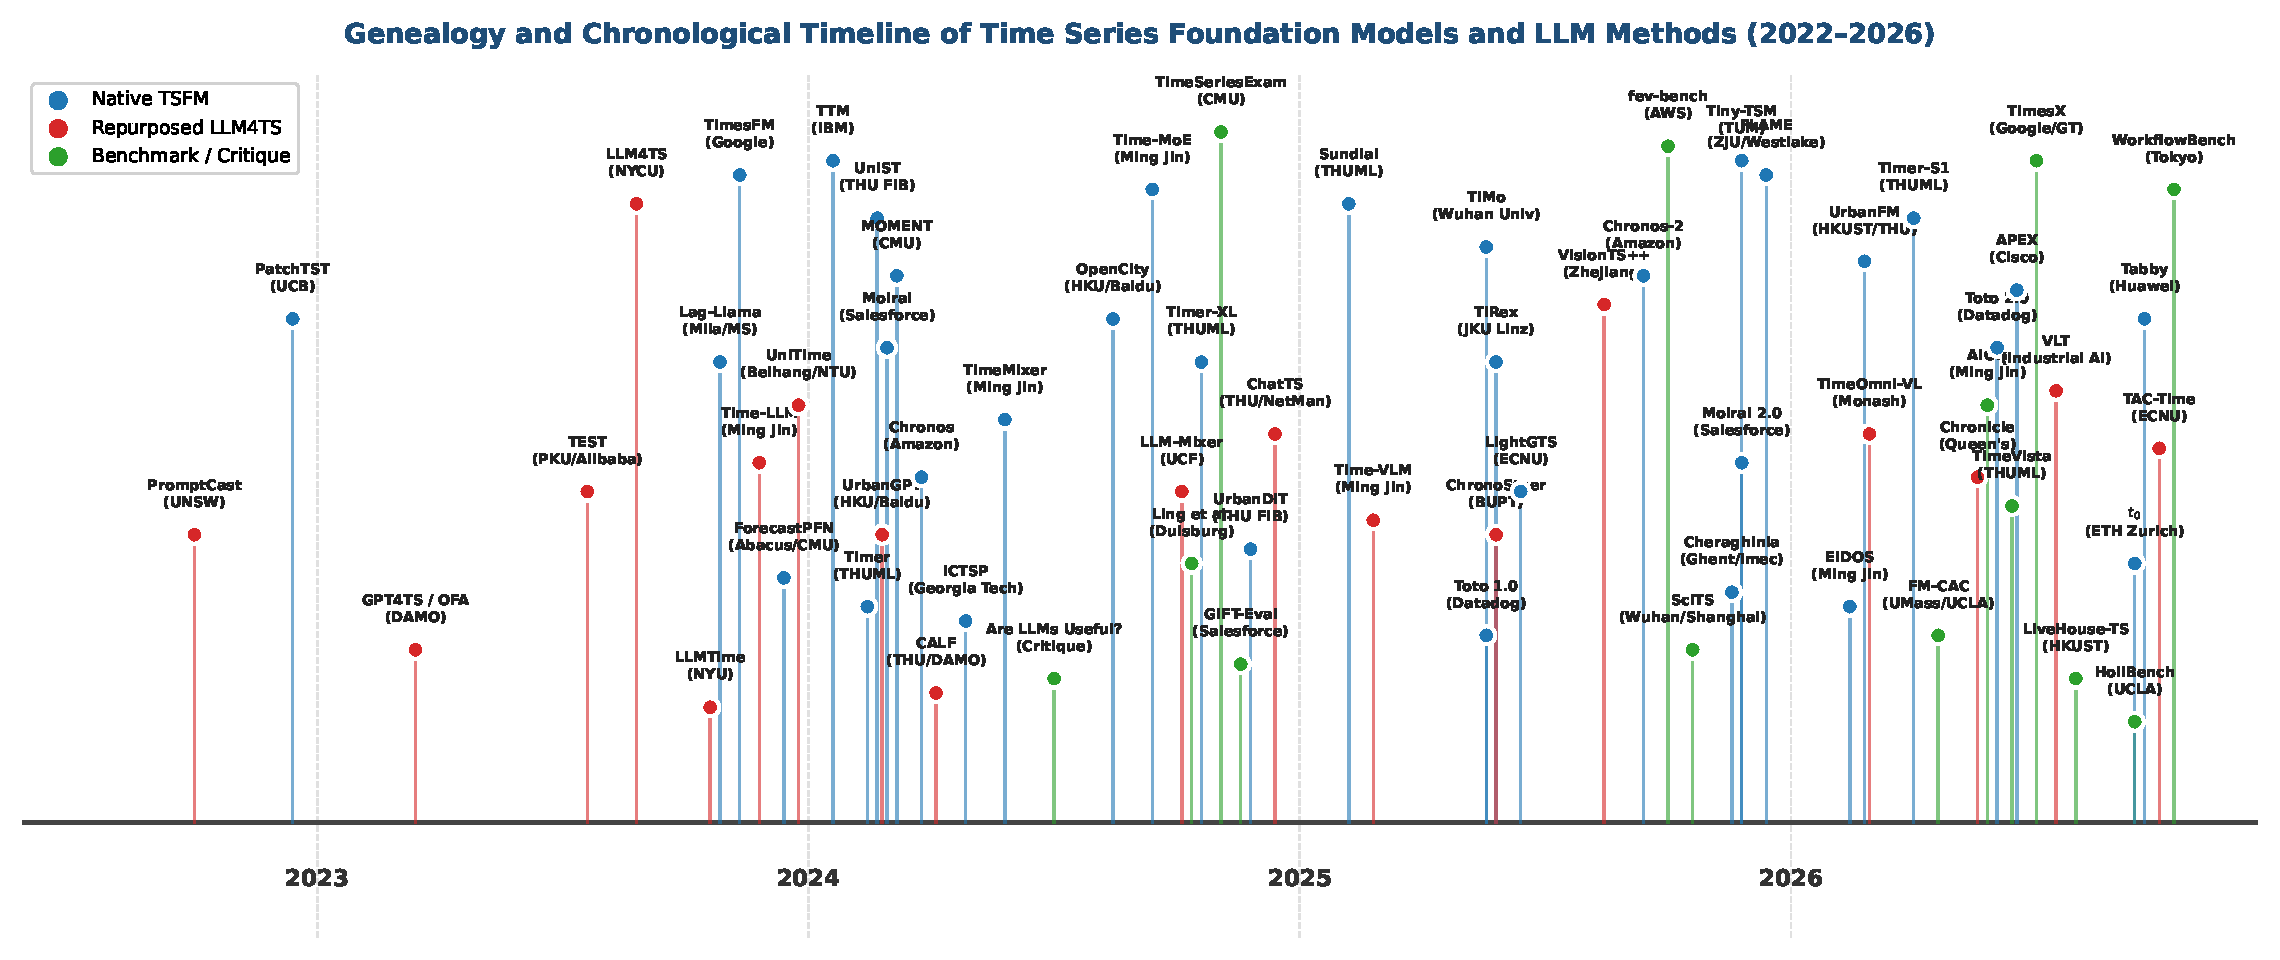
\includegraphics[width=0.98\textwidth]{figures/fig_timeline.pdf}
\caption{Genealogy and chronological release timeline of representative time series foundation models and repurposed language model frameworks from 2022 to 2026.}
\label{fig:timeline}
\end{figure*}

\subsection{Critical Perspectives: Are LLMs Actually Useful for Time Series?}

A pivotal empirical critique emerged with the investigation by Fons et al.~\cite{fons2024arellmsuseful}, entitled \emph{``Are Language Models Actually Useful for Time Series Forecasting?''}
Through extensive ablation experiments across multiple LLM-based forecasters (including GPT4TS~\cite{zhou2023onefitsall} and Time-LLM~\cite{jin2023timellm}), the authors isolated the impact of pre-trained language weights by comparing:
\begin{enumerate}[leftmargin=*]
    \item Frozen pre-trained language weights (e.g., GPT-2, Llama-2);
    \item Randomly initialized transformer weights with the same architecture;
    \item Compact specialized baselines (such as PatchTST~\cite{nie2023patchtst} and lightweight MLPs).
\end{enumerate}

Their empirical findings revealed striking conclusions:
\begin{itemize}[leftmargin=*]
    \item Replacing pre-trained language weights with \emph{randomly initialized weights} resulted in comparable, and in several cases superior, forecasting accuracy.
    \item Much of the empirical gains reported in early LLM4TS literature originated from the structural benefits of \emph{subseries patching} and normalization, rather than any semantic or temporal reasoning inherent in linguistic pre-training.
    \item In terms of operational efficiency, frozen $7\text{B}$ parameter language models require up to $100\times$ more memory and $50\times$ longer inference latency than compact native models like TTM~\cite{ekambaram2024ttm} ($8\text{M}$ parameters) or Timer~\cite{liu2024timer} ($84\text{M}$ parameters), which consistently achieve competitive or superior accuracy.
\end{itemize}

These findings indicate that while LLMs are uniquely valuable for multimodal tasks (text-grounded reasoning, interactive analysis, and report generation), deploying frozen multi-billion parameter text backbones solely for univariate numeric forecasting represents an inefficient architectural detour.

\begin{figure*}[t]
\centering
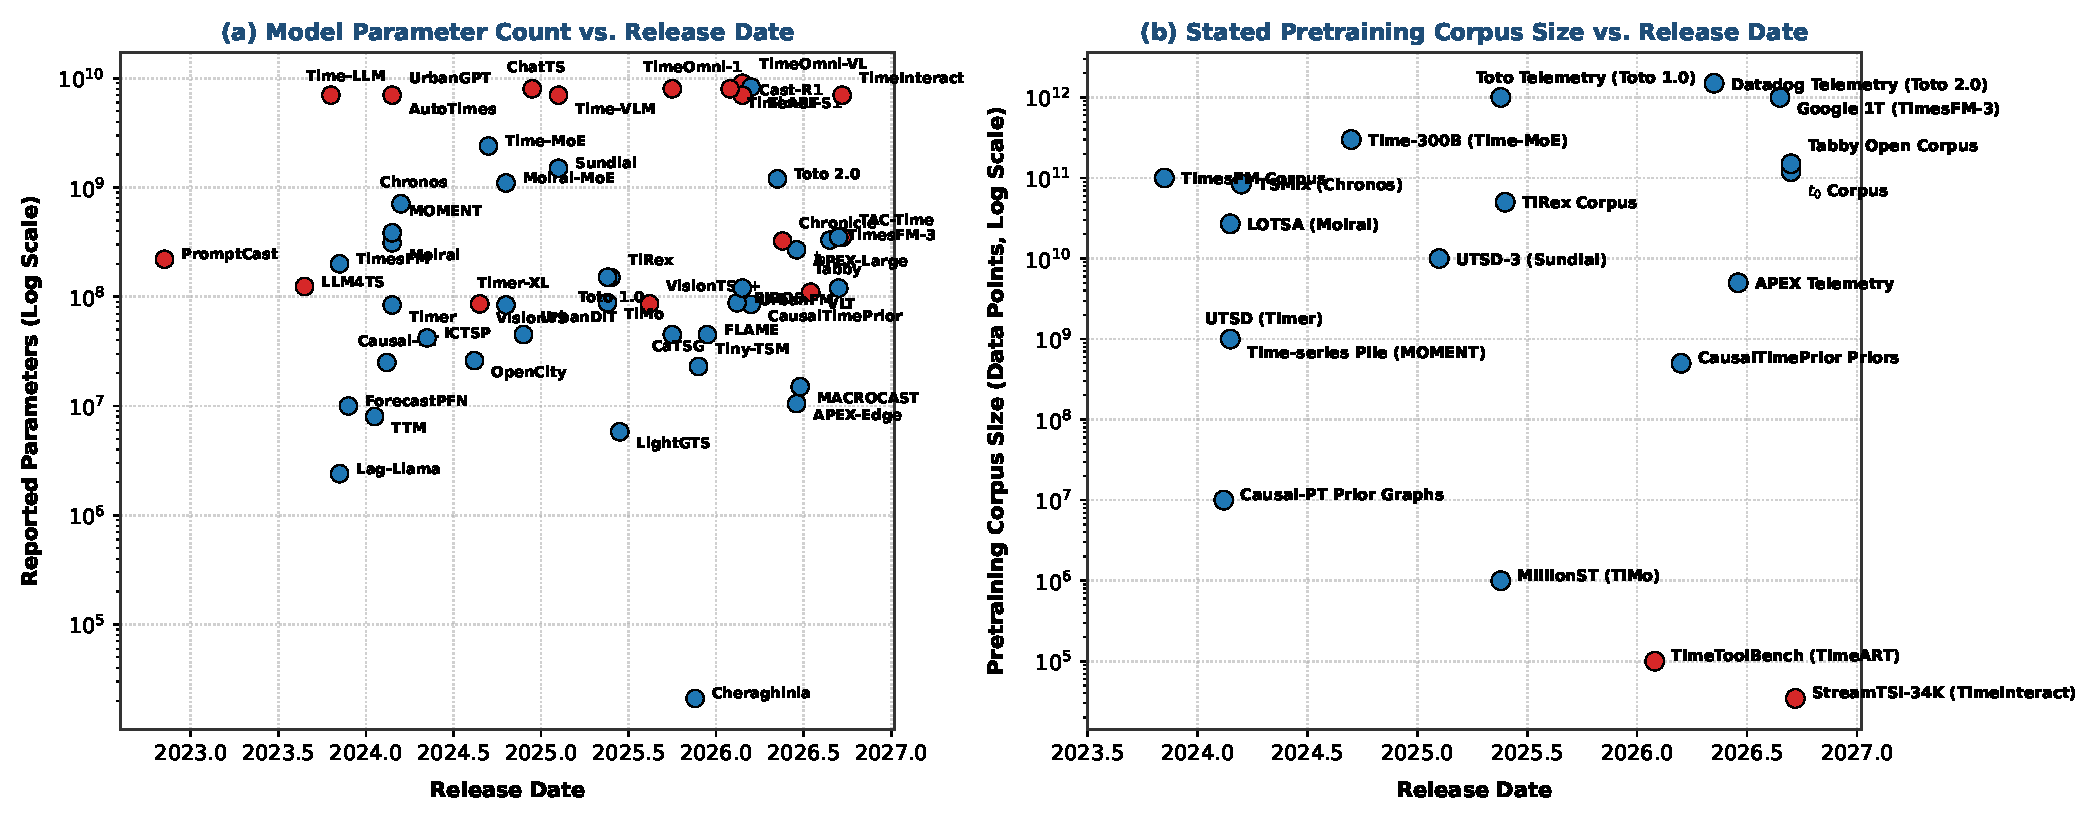
\includegraphics[width=0.98\textwidth]{figures/fig_params_corpus.pdf}
\caption{Scaling dynamics across the literature: (a) Reported parameter counts vs. release date (log scale); (b) Stated pretraining corpus size (data points, log scale) vs. release date.}
\label{fig:params_corpus}
\end{figure*}

\subsection{Data Contamination, Temporal Leakage, and Probabilistic Reliability}

\subsubsection{Benchmark Contamination Audits}
A critical vulnerability in contemporary foundation model evaluation is \emph{benchmark contamination}. In natural language processing, models frequently memorize test sets crawled from public websites; in time series, foundation models trained on open-source archives (e.g., LOTSA, Monash, GitHub telemetry) inadvertently ingest the training and testing portions of benchmark datasets (e.g., ETT, Weather)~\cite{gong2025rethinkingeval}.

Gong et al.~\cite{gong2025rethinkingeval} systematically audited 12 major foundation models and discovered widespread temporal overlap between pretraining datasets and standard test benchmarks. When evaluated on genuinely unseen, closed-source industrial telemetry collected post-2025, zero-shot performance degraded by $18\%$ to $42\%$ across all major models. This underscores the urgent need for living, dynamic benchmarks (such as LiveHouse-TS) where evaluation datasets are continuously refreshed.

\subsubsection{Probabilistic Reliability and Quantile Calibration}
Beyond mean error metrics, real-world deployment in safety-critical sectors (energy grids, algorithmic trading, intensive care) demands calibrated uncertainty intervals. In a recent rigorous audit, Li et al.~\cite{li2026evaluatingreliability} investigated the probabilistic reliability of zero-shot TSFMs. Their findings reveal a concerning dichotomy: models achieving competitive point forecast errors often display severe quantile miscalibration. Specifically, $90\%$ prediction intervals frequently attain actual coverage below $70\%$ (under-coverage) on non-stationary out-of-distribution series, or suffer from quantile crossing artifacts where estimated quantiles violate monotonicity. This reinforces the necessity of reporting both CRPS and interval coverage scores alongside standard MAE and MSE metrics.

\begin{figure*}[t]
\centering
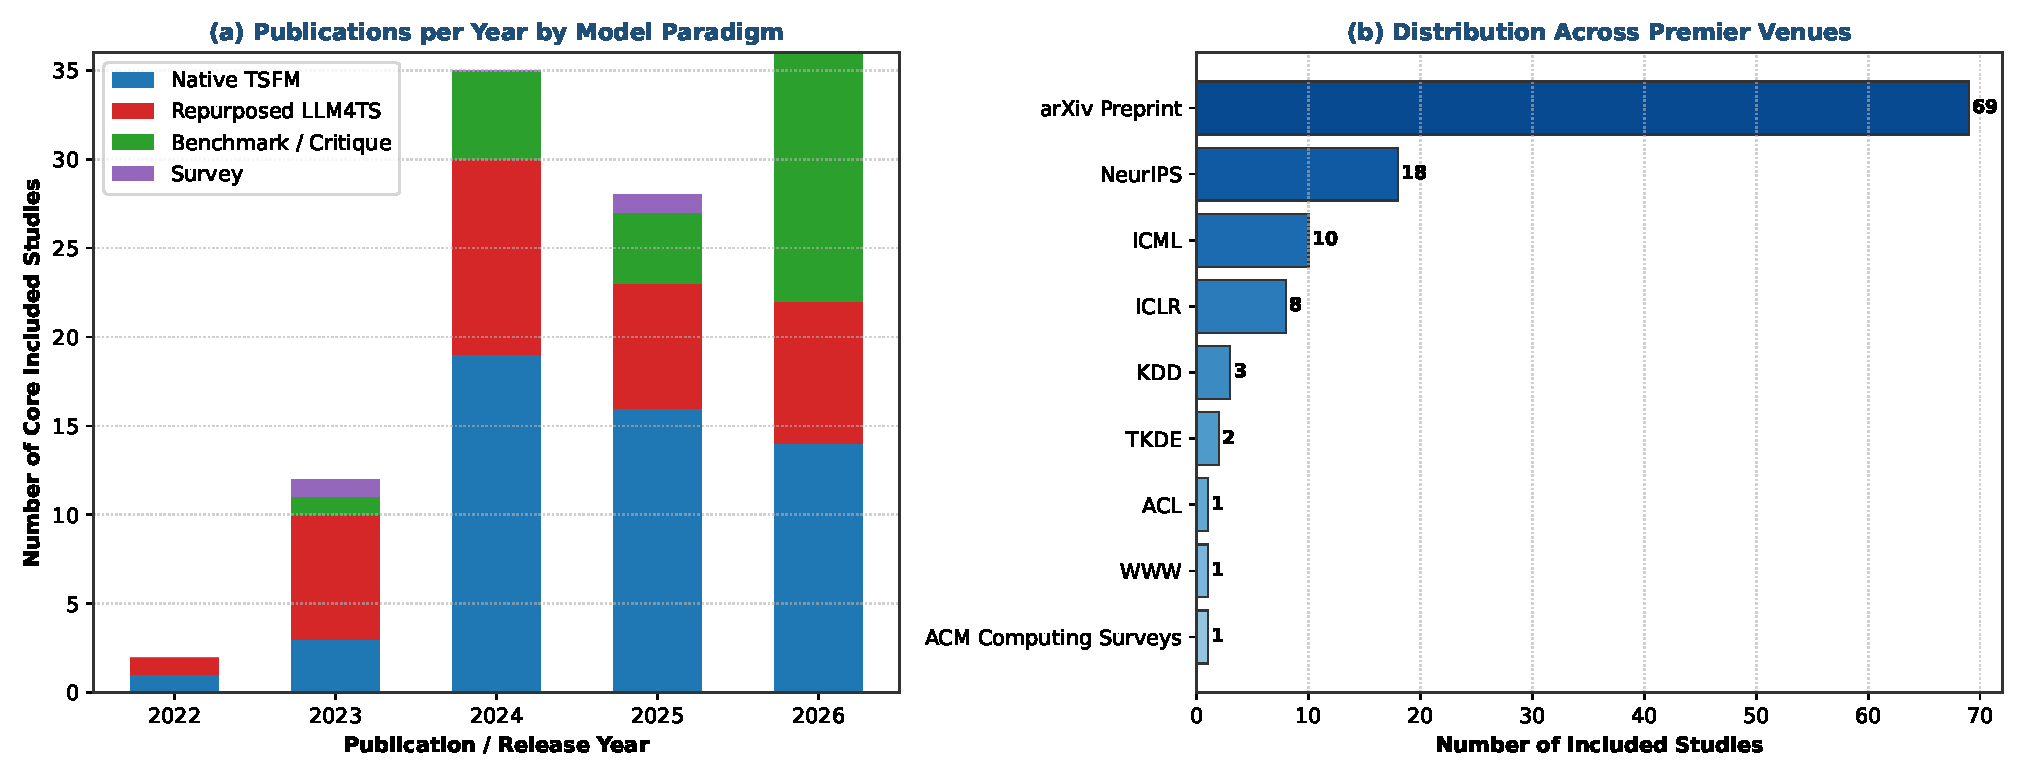
\includegraphics[width=0.98\textwidth]{figures/fig_category_dist.pdf}
\caption{Meta-review statistics: (a) Publications per year broken down by model paradigm (stacked bar chart); (b) Distribution of included studies across premier peer-reviewed venues.}
\label{fig:category_dist}
\end{figure*}

\subsection{Empirical Scaling Laws in Temporal Data}

Do foundation models for time series exhibit the predictable power-law scaling observed in NLP?
Recent empirical studies on large pre-trained models—notably Time-MoE~\cite{shi2024timemoe} ($2.4\text{B}$ parameters, $300\text{B}$ points), Sundial~\cite{thuml2025sundial} ($1.5\text{B}$ parameters), Timer-S1~\cite{thuml2026timers1} ($8.3\text{B}$ parameters), and Toto 2.0~\cite{datadog2026toto2} ($2.5\text{B}$ parameters)—demonstrate that when data quality and volume are rigorously maintained, test loss follows power-law scaling as a function of compute and dataset tokens:
\begin{equation}
    L(N, D) = \left( \frac{N_c}{N} \right)^{\alpha_N} + \left( \frac{D_c}{D} \right)^{\alpha_D} + L_0.
\end{equation}
However, unlike text, scaling parameters without expanding temporal diversity leads to rapid overfitting. Cross-domain pretraining on synthetic kernel mixtures and diverse physical systems is essential to sustain positive scaling exponents.

\section{Open Challenges and Future Horizons}
\label{sec:outlook}

Despite rapid progress in foundation models and LLM adaptations, temporal machine learning remains in a formative phase. In this section, we delineate six critical open research horizons that must be addressed to achieve truly universal temporal intelligence.

\subsection{Irregular Sampling and Continuous-Time Dynamics}
Existing foundation models (e.g., Chronos, TimesFM, MOIRAI) predominantly assume regularly sampled, synchronous discrete grids. However, real-world physical telemetry—such as ICU medical records, IoT sensor dropouts, and financial trade ticks—arrives at asynchronous, irregular time intervals.
Emerging approaches such as FlowState~\cite{king2025flowstate} leverage continuous flow matching and continuous-time neural state-space models to achieve sampling-rate equivariance. Future foundation architectures must natively encode irregular time intervals $(\Delta t)$ into latent manifolds rather than relying on crude imputation or resampling heuristics.

\subsection{Prior-Data Fitted Bayesian Networks}
Standard foundation models require thousands of gradient optimization steps during fine-tuning. A compelling alternative is demonstrated by TabPFN-TS~\cite{muller2025tabpfnts}, which adapts Prior-Data Fitted Networks to time series. By training a transformer exclusively on synthetic prior stochastic processes (e.g., Gaussian processes, Ornstein-Uhlenbeck, and Markov switching models), the network learns to perform Bayesian posterior inference in a single forward pass without parameter updates. Expanding synthetic prior spaces to encompass complex non-linear dynamics represents a fertile research direction.

\subsection{Extreme Long-Horizon Context and Serial Scaling}
In natural language, modern models handle context windows exceeding $1\text{M}$ tokens. In temporal analysis, historical series often span millions of high-frequency timestamps. Capturing decadal climate shifts, annual retail cycles, and second-level power grid vibrations within a single context window demands extreme context scaling. Architectural innovations such as long-context state-space models (Mamba), hierarchical linear attention, and serial scaling (as explored in Timer-XL~\cite{liu2024timerxl} and Timer-S1~\cite{thuml2026timers1}) will be essential to eliminate context truncation.

\subsection{Unified Multimodal Perception}
Real-world decision-making rarely relies on isolated scalar numbers. An industrial operator monitors pressure gauges alongside diagnostic maintenance logs; a macroeconomist reads financial reports while analyzing stock tickers; an environmental scientist tracks satellite imagery across seasonal vegetation cycles~\cite{qin2025timo}. Future foundation models must advance beyond ad-hoc text reprogramming to train native multi-modal architectures from scratch—treating numerical time series, textual reports, spatial optical imagery, and spectral vibrations as co-equal perceptual modalities, as pioneered by Chronicle~\cite{quinlan2026chronicle}, VLT~\cite{wang2026vlt}, and ChronoSteer~\cite{wang2025chronosteer}.

\subsection{Calibrated Uncertainty under Distribution Shift}
In safety-critical applications (such as healthcare and grid management), an uncalibrated point forecast is hazardous. As demonstrated by recent reliability audits~\cite{li2026evaluatingreliability}, current zero-shot models frequently underestimate predictive variance when confronted with unprecedented macroeconomic shocks or extreme weather events. Developing conformal prediction techniques, robust Bayesian heads, and flow-based generative sampling that maintain rigorous coverage guarantees under out-of-distribution shifts is imperative.

\subsection{Edge Deployment, Hardware Quantization, and Green AI}
While research models scale to billions of parameters, industrial IoT environments require deployment on low-power microcontrollers, edge gateways, and automotive Electronic Control Units (ECUs). Systematic cross-platform benchmarking (HoliBench~\cite{chakrabarti2026holibench}), integer mixed-precision quantization (INT8/INT4 on embedded FPGAs~\cite{ling2024resource}), ultra-compact patch encoders~\cite{cheraghinia2025lightweight,birkel2025tinytsm}, and carbon-aware battery-buffered dynamic dispatch (FM-CAC~\cite{yang2026fmcac}) will be essential to transform temporal foundation research into sustainable, energy-efficient cyber-physical systems.

\subsection{Autonomous Living Foundations and Continuous Discovery}
With dozens of new preprints posted weekly across machine learning repositories, academic surveys quickly become obsolete. Future research must embrace autonomous, living benchmark harnesses (e.g., LiveHouse-TS~\cite{wen2026livehouse}) and continuous automated snowballing pipelines that monitor arXiv and Semantic Scholar streams, evaluate newly dropped weights against standardized multi-granularity leakage audits (It's TIME~\cite{qiao2026time}), and iteratively update systematic taxonomies.


\section{Conclusion}
\label{sec:conclusion}

In this survey, conducted under the PRISMA 2020 systematic review protocol, we have synthesized the foundational developments at the intersection of Large Language Models and Time Series Foundation Models from 2021 through 2026. We formalized mathematical definitions of temporal sequences, subseries patching, and quantization; introduced a unified five-dimensional taxonomy; and compared 41 core benchmark and foundation models across architecture, tokenization, pretraining corpora, and uncertainty formulations.

Our critical synthesis highlights a decisive architectural demarcation:
\begin{itemize}[leftmargin=*]
    \item \emph{Native TSFMs} (such as Chronos, TimesFM, MOIRAI, Timer, and TTM) demonstrate superior parameter efficiency, faster inference latency, and stronger zero-shot numeric forecasting accuracy by training directly on temporal dynamics without linguistic mismatch.
    \item \emph{Repurposed LLMs} (such as Time-LLM and multimodal reasoning frameworks) excel not at raw numeric extrapolation, but as cognitive orchestrators—grounding numerical time series within textual narratives, metadata, and decision-support systems.
\end{itemize}

Looking ahead, the frontier of temporal intelligence lies in resolving benchmark contamination, achieving continuous-time sampling equivariance, calibrating uncertainty under non-stationary shifts, and delivering ultra-efficient edge deployment. We hope this survey provides a rigorous compass for researchers and practitioners building the next generation of universal temporal models.


\bibliographystyle{IEEEtran}
\bibliography{references}

\end{document}
